\documentclass{beamer}
\usetheme{Boadilla}
\setbeamertemplate{navigation symbols}{} % To remove the navigation symbols from the bottom of all slides uncomment this line

%------------------------------------------------
% Colors
\usepackage{xcolor}	 % Required for custom colors
% Define a few colors for making text stand out within the presentation
\definecolor{mygreen}{RGB}{44,85,17}
\definecolor{myblue}{RGB}{34,31,217}
\definecolor{mybrown}{RGB}{194,164,113}
\definecolor{myred}{RGB}{255,66,56}
% Use these colors within the presentation by enclosing text in the commands below
\newcommand*{\mygreen}[1]{\textcolor{mygreen}{#1}}
\newcommand*{\myblue}[1]{\textcolor{myblue}{#1}}
\newcommand*{\mybrown}[1]{\textcolor{mybrown}{#1}}
\newcommand*{\myred}[1]{\textcolor{myred}{#1}}
%------------------------------------------------
\setbeamercolor{structure}{fg=mygreen}
%------------------------------------------------
\setbeamertemplate{itemize item}{\scriptsize\raise1.25pt\hbox{\donotcoloroutermaths$\blacktriangleright$}}
\setbeamertemplate{itemize subitem}{\tiny\raise1.5pt\hbox{\donotcoloroutermaths$\blacktriangleright$}}
\setbeamertemplate{itemize subsubitem}{\tiny\raise1.5pt\hbox{\donotcoloroutermaths$\blacktriangleright$}}


%------------------------------------------------
% Fonts
%------------------------------------------------
\usepackage[T1]{fontenc}	 % For correct hyphenation and T1 encoding
\usepackage{lmodern} % Default font: latin modern font
\renewcommand{\familydefault}{\sfdefault} % Sans serif - this may need to be commented to see the alternative fonts
%------------------------------------------------

%------------------------------------------------
% Various required packages
%-----------------------------------------------


\usepackage     [utf8]          {inputenc}
\usepackage     [T1]            {fontenc}
\usepackage                     {color}
\usepackage                     {amsmath}
\usepackage                     {graphicx}
\usepackage     [english]       {babel}
\usepackage                     {natbib}
\usepackage                     {hyperref}
\usepackage						{cleveref}
\usepackage						{subfigure}
\usepackage						{multirow}
\usepackage						{booktabs} % Allows the use of \toprule, \midrule and \bottomrule in tables
\usepackage						{tikz}
\usepackage						{multicol} % Required for creating multiple columns in slides

%------------------------------------------------
\newcommand{\topline}{%
  \tikz[remember picture,overlay] {%
    \draw[mygreen,very thick] ([yshift=-1.7cm]current page.north west)
             -- ([yshift=-1.7cm,xshift=11cm]current page.north west);}}
%------------------------------------------------
% Slide layout configuration

\setbeamertemplate{frametitle}
{	
	\huge
	\vspace*{0.3cm}
    \insertframetitle  \\
     \tikz[remember picture,overlay] {%
        \draw[mygreen,very thick] ([yshift=-1.7cm]current page.north west)
                 -- ([yshift=-1.7cm,xshift=11cm]current page.north west);}
     
  %  \insertframesubtitle
}
%\AtBeginDocument{\renewcaptionname{english}{\contentsname}{\Large Agenda}} 
%Title
%------------------------------------------------
\title[]{RETRIEVAL ADVANCES OF BrO/SO2 MOLAR RATIOS FROM NOVAC} % The short title appears at the bottom of every slide, the full title is only on the title page

\author{Elsa Wilken} % Your name
\institute[] % Your institution as it will appear on the bottom of every slide, may be shorthand to save space
{
Master Thesis \\ % Your institution for the title page
\medskip
%\textit{e.wilken@yahoo.de} % Your email address
}
\date{\today} % Date, can be changed to a custom date




\begin{document}

%------------------------------------------------
%	TITLE SLIDE
%------------------------------------------------
\begin{frame}
\titlepage
\end{frame}


%------------------------------------------------
%	Established Routine
%------------------------------------------------

%------------------------------------------------
%	Contamination Problem
%------------------------------------------------
\frame{
\frametitle{Contamination Problem}
	\begin{multicols}{2}
		\begin{itemize}
			 \item 10$\%$  of the Data are contaminated in Nevado Del Ruiz
			\item 6.4$\%$  of the Data are contaminated in Tungurhua
		\end{itemize}
		In the following we only work with the contaminated data
		\begin{minipage}[t]{0.5\textwidth}
			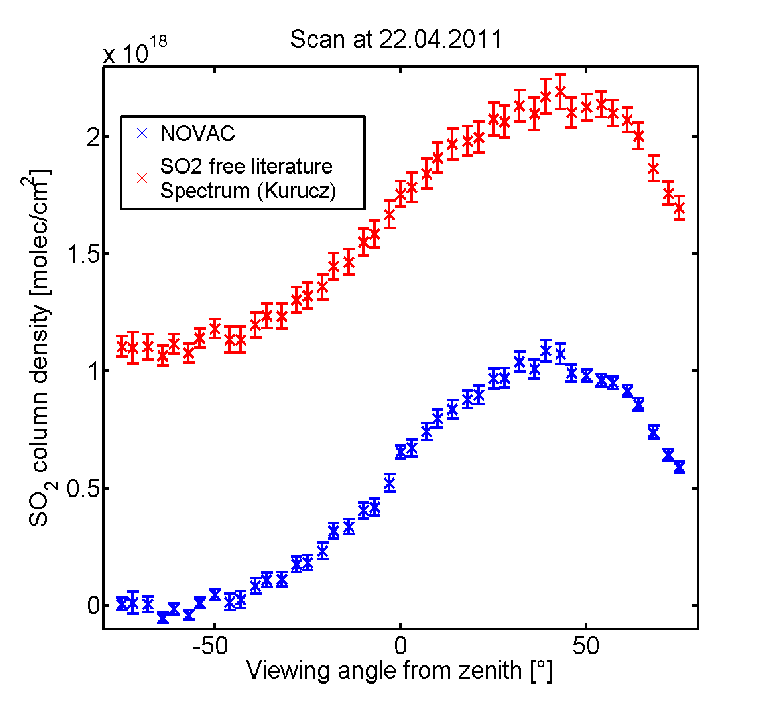
\includegraphics[width=\textwidth]{./Bilder/contaminated}
		\end{minipage}
	\end{multicols}
}
%------------------------------------------------
%	BrO Error dependency on variables
%------------------------------------------------
\frame{
\frametitle{BrO Error Tungurhua /Nevado Del Ruiz}
	\begin{figure}[h!]			
	\subfigure[Data of Tungurahua]{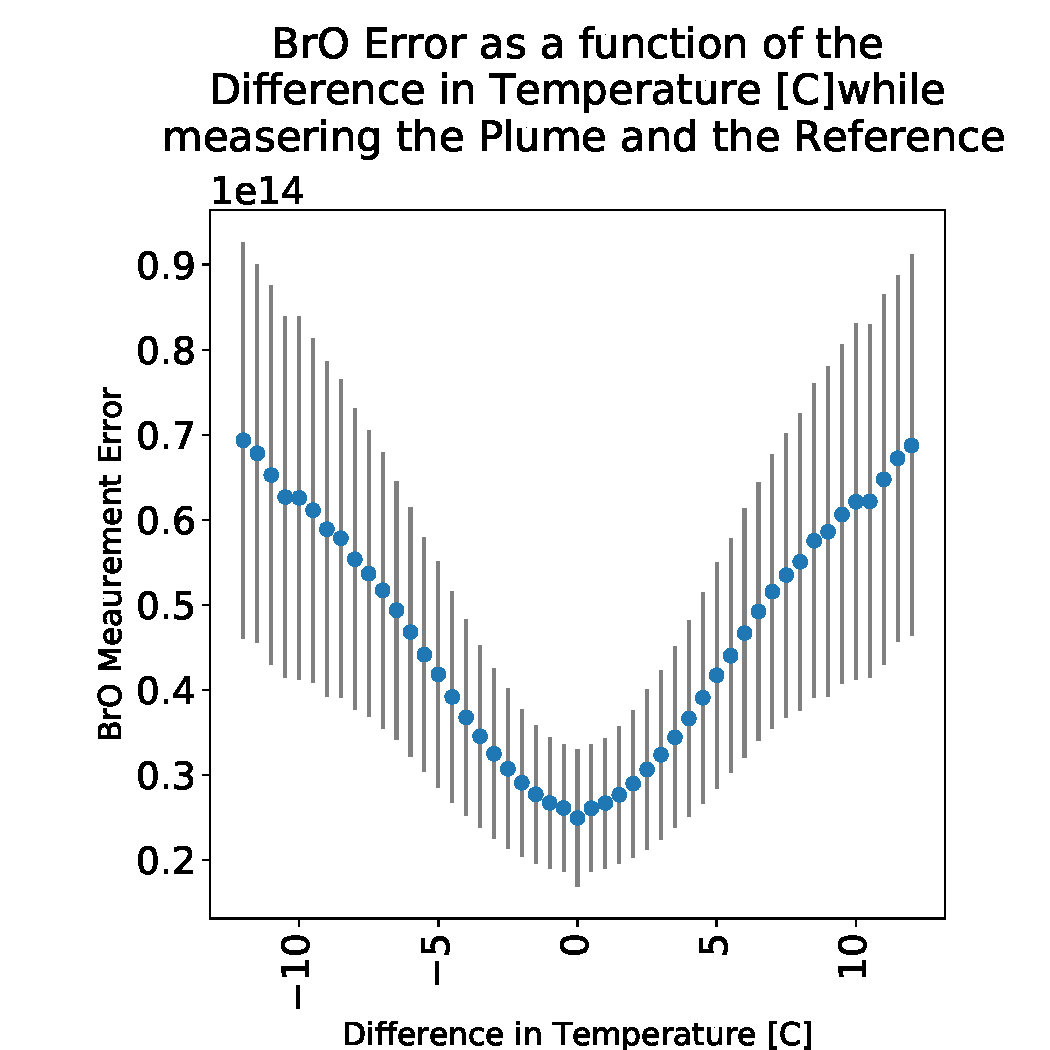
\includegraphics[width=0.49\textwidth]{Bilder/DiffTemp_Tungu}}
	\subfigure[Data of Nevado Del Riz]{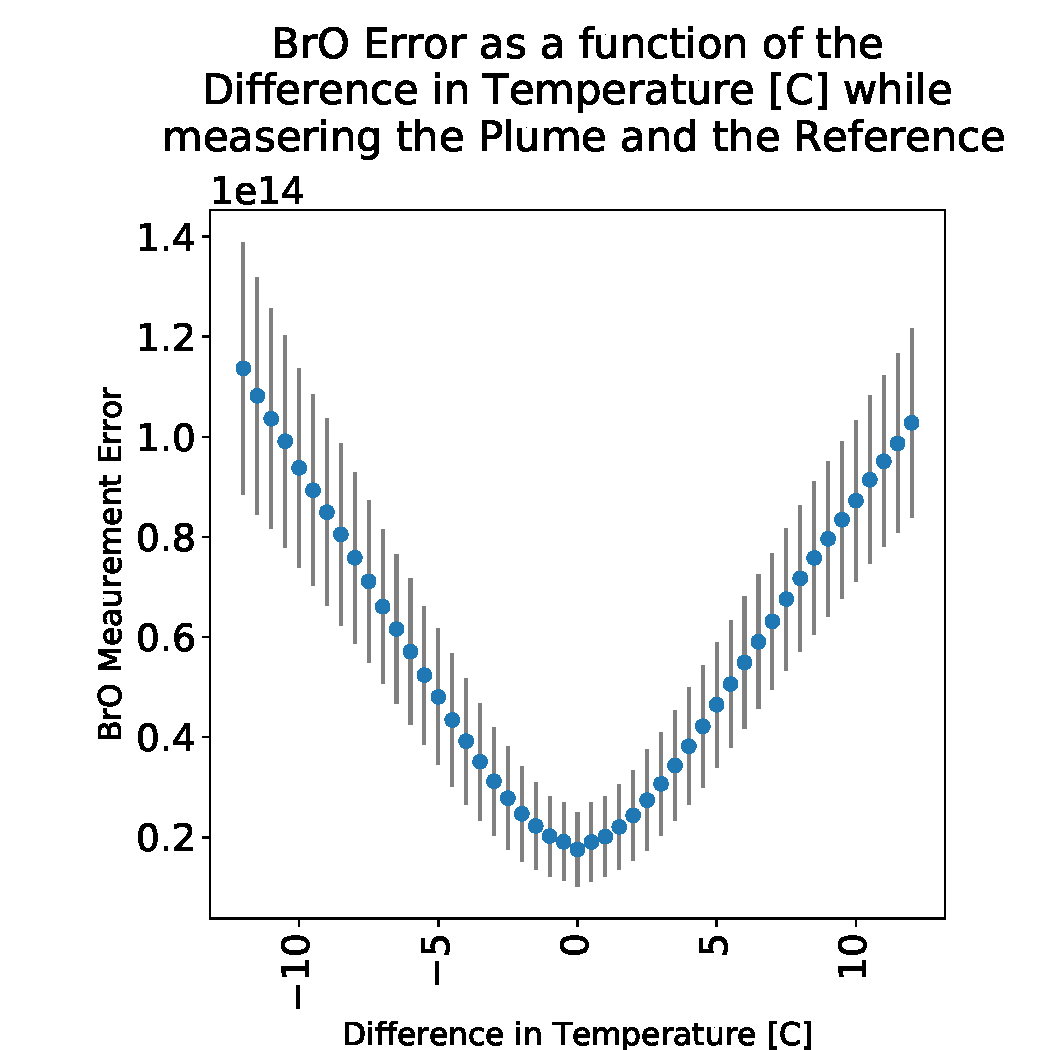
\includegraphics[width=0.49\textwidth]{Bilder/DiffTemp_Nevad}}
	\caption{Titel unterm gesamten Bild}
	\label{fig:difftemp}
\end{figure}[h!]
\begin{itemize}
	\item The BrO error has the strongest dependence on the temperature difference. At Tungurahua (Nevado Del Ruiz) the BrO error increases by factor of $3.53\cdot10^{12}$  per degree.
	\begin{align*}
	\rightarrow&  BrO_{Error} = f(ext. P)+ 3.53\cdot10^{12}\cdot\frac{\Delta T}{1C^{\circ}} + \mathcal{O}\left(\right) & Tungurahua\\
	\rightarrow&  BrO_{Error} = f(ext. P)+7.56\cdot10^{12}\cdot\frac{\Delta T}{1C^{\circ}} + \mathcal{O}\left(\right) & Nevado Del Ruiz\\
	\end{align*}
\end{itemize}
}
\frame{
	\frametitle{BrO Error Tungurhua /Nevado Del Ruiz}
	\begin{figure}[h!]			
		\subfigure[Data of Tungurahua]{\includegraphics[width=0.49\textwidth]{Bilder/Diffdaytime_Tungu}}
		\subfigure[Data of Nevado Del Riz]{\includegraphics[width=0.49\textwidth]{Bilder/Diffdaytime_Nevad}}
		\caption{Titel unterm gesamten Bild}
		\label{fig:diffdaytime}
	\end{figure}
	\begin{itemize}
		\item We found a dependency of the BrO error on the daytime. We assume, that this dependency comes from other external parameters which change during the day. 
		\item The BrO Error increases with the daytime differences like: \\
		\begin{align*}
		\rightarrow&  BrO_{Error} = f(ext. P)+1.33\cdot10^{12}\cdot\frac{\Delta DT}{1h}  + \mathcal{O}\left(\right)& Tungurahua\\
		\rightarrow&  BrO_{Error} = f(ext. P)+1.58\cdot10^{13}\cdot\frac{\Delta DT}{1h} + \mathcal{O}\left(\right) & Nevado Del Ruiz\\
		\end{align*}
		
	\end{itemize}
}
\frame{
	\frametitle{BrO Error Tungurhua /Nevado Del Ruiz}
		\begin{figure}[h]		
		\subfigure[Data of Tungurahua]{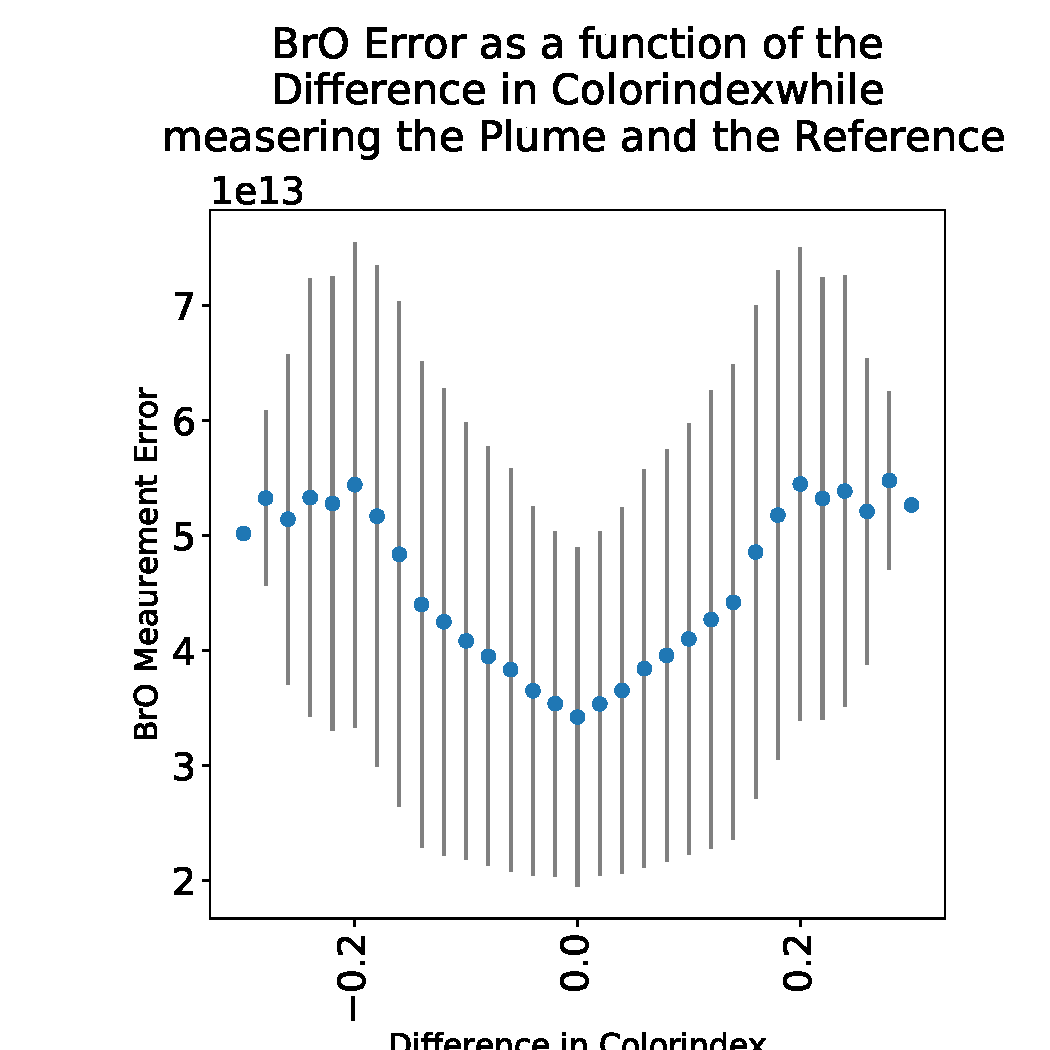
\includegraphics[width=0.49\textwidth]{Bilder/DiffColidx_Tungu}}
		\subfigure[Data of Nevado Del Riz]{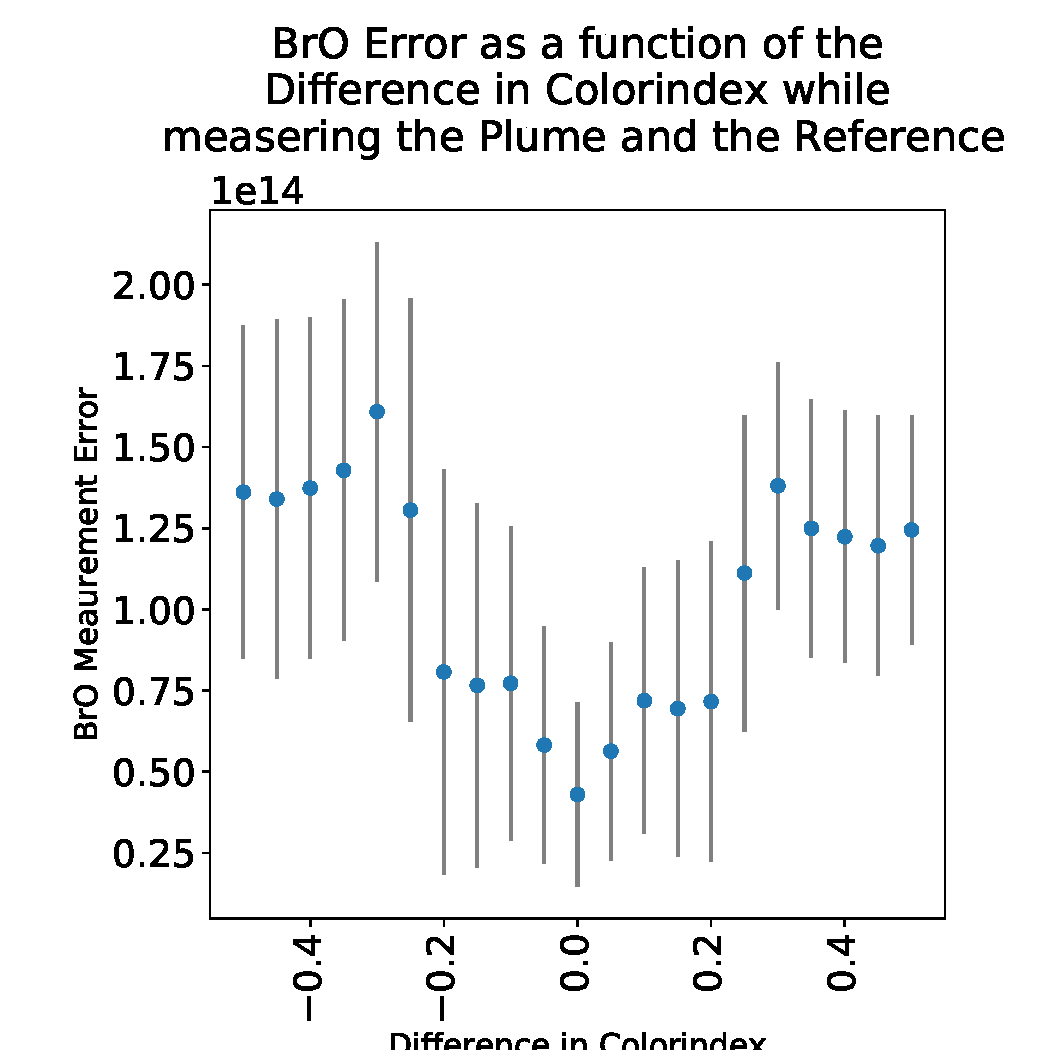
\includegraphics[width=0.49\textwidth]{Bilder/DiffColidx_Nevad}}
		\caption{Titel unterm gesamten Bild}
		\label{fig:diffcolidx}
	\end{figure}
	\begin{itemize}
	\item 	The BrO Error increases with the Colorindex differences as \\
	\begin{align*}
	\rightarrow&  BrO_{Error} = f(ext. P)+ 1.01\cdot10^{13}\cdot\frac{\Delta Cidx}{0.1} + \mathcal{O}\left(\right) & Tungurahua\\
	\rightarrow&  BrO_{Error} = f(ext. P)+  4\cdot10^{13}\cdot\frac{\Delta Cidx}{0.1} + \mathcal{O}\left(\right) & Nevado Del Ruiz\\
	\end{align*}
\end{itemize}
}
\frame{
	\frametitle{BrO Error Tungurhua /Nevado Del Ruiz}
	\begin{figure}[h!]			
	\subfigure[Data of Tungurahua]{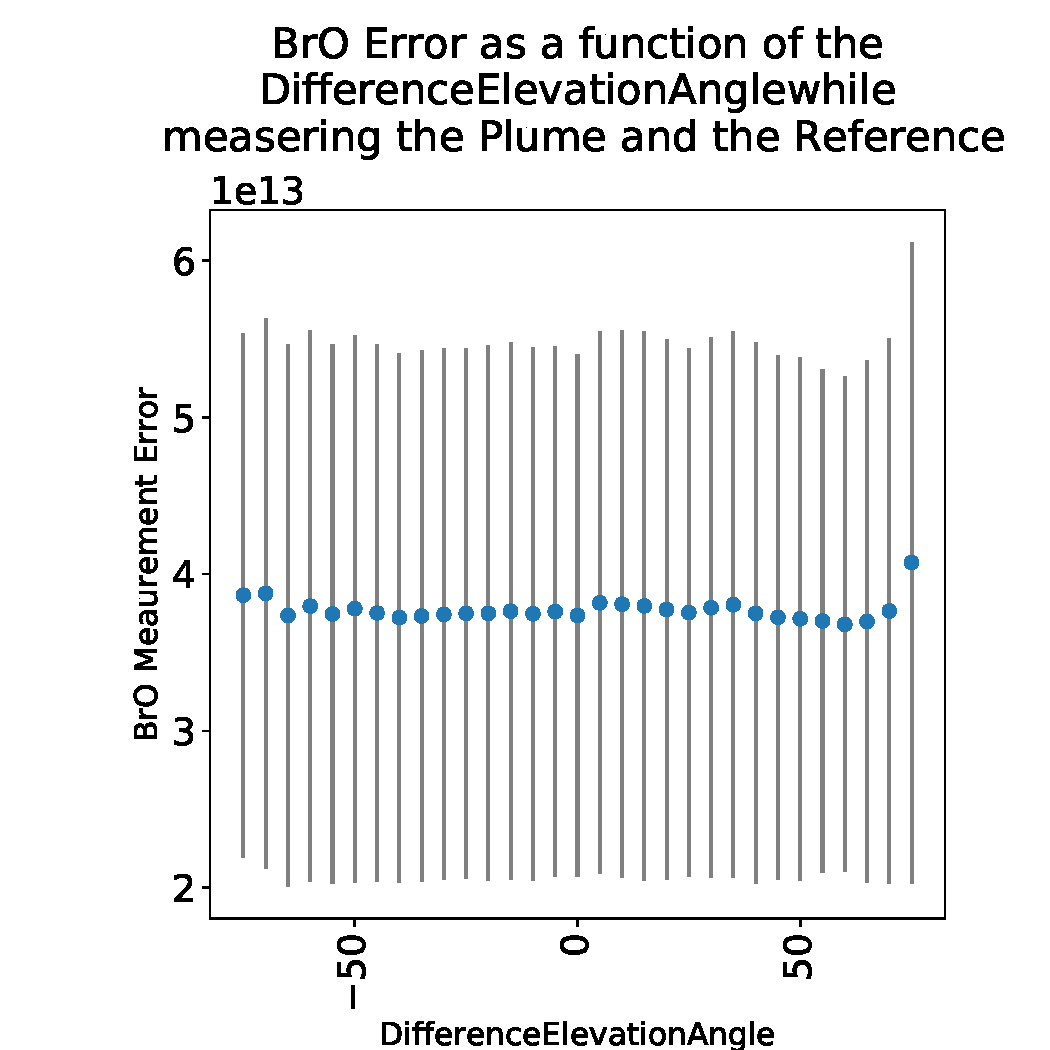
\includegraphics[width=0.49\textwidth]{Bilder/DiffElevAngle_Tungu}}
	\subfigure[Data of Nevado Del Riz]{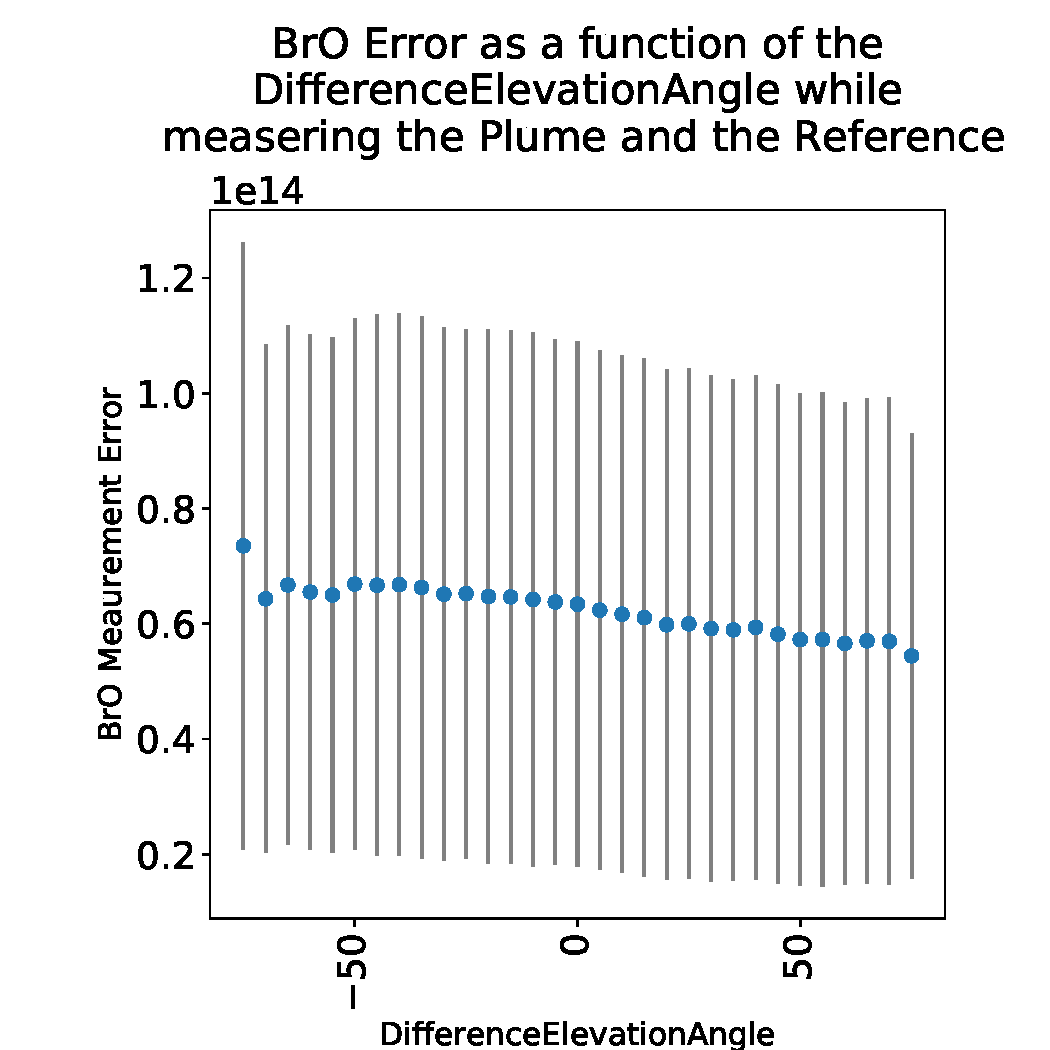
\includegraphics[width=0.49\textwidth]{Bilder/DiffElevAngle_Nevad}}
	\caption{Titel unterm gesamten Bild}
\end{figure}
}
\frame{
	\frametitle{BrO Error Tungurhua /Nevado Del Ruiz}
\begin{figure}		
	\subfigure[Data of Tungurahua]{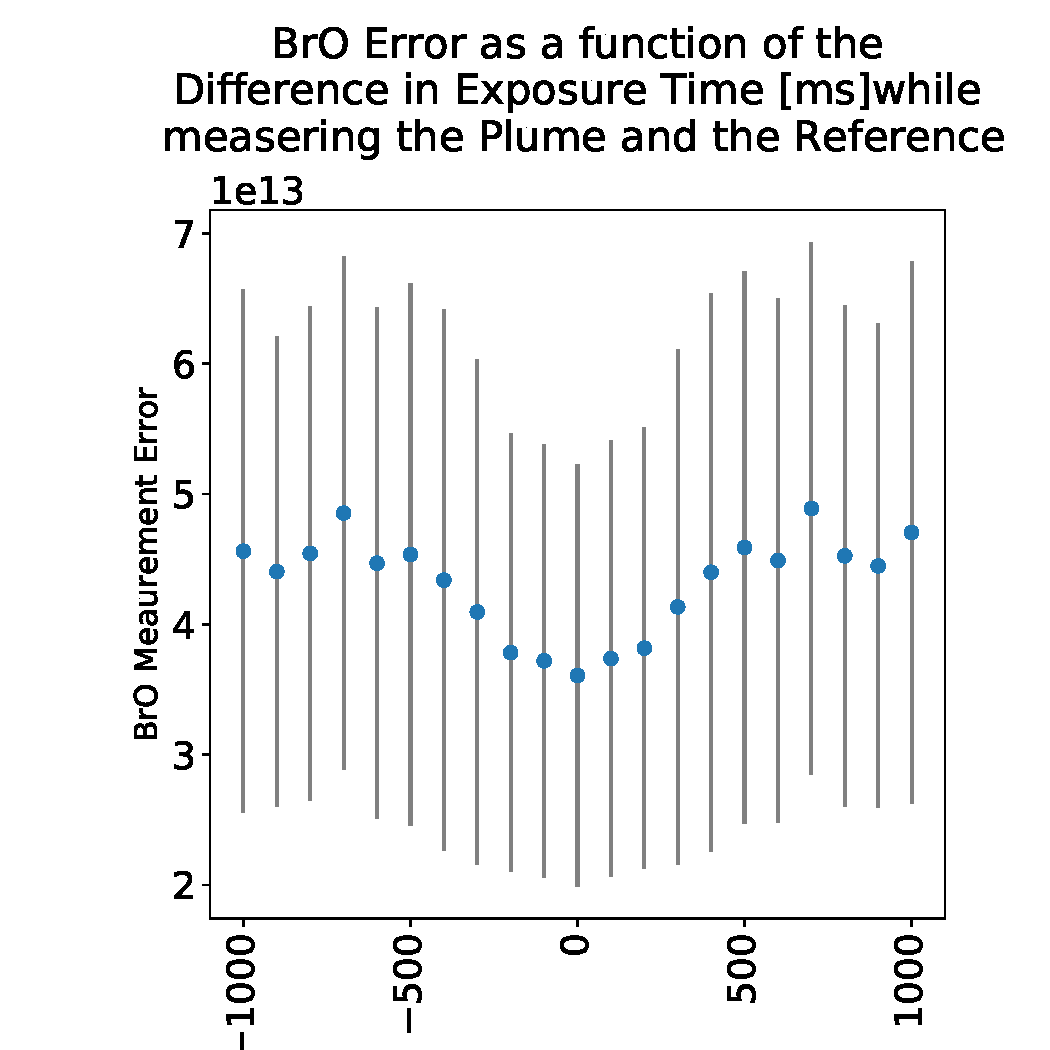
\includegraphics[width=0.49\textwidth]{Bilder/DiffExpTime_Tungu}}
	\subfigure[Data of Nevado Del Riz]{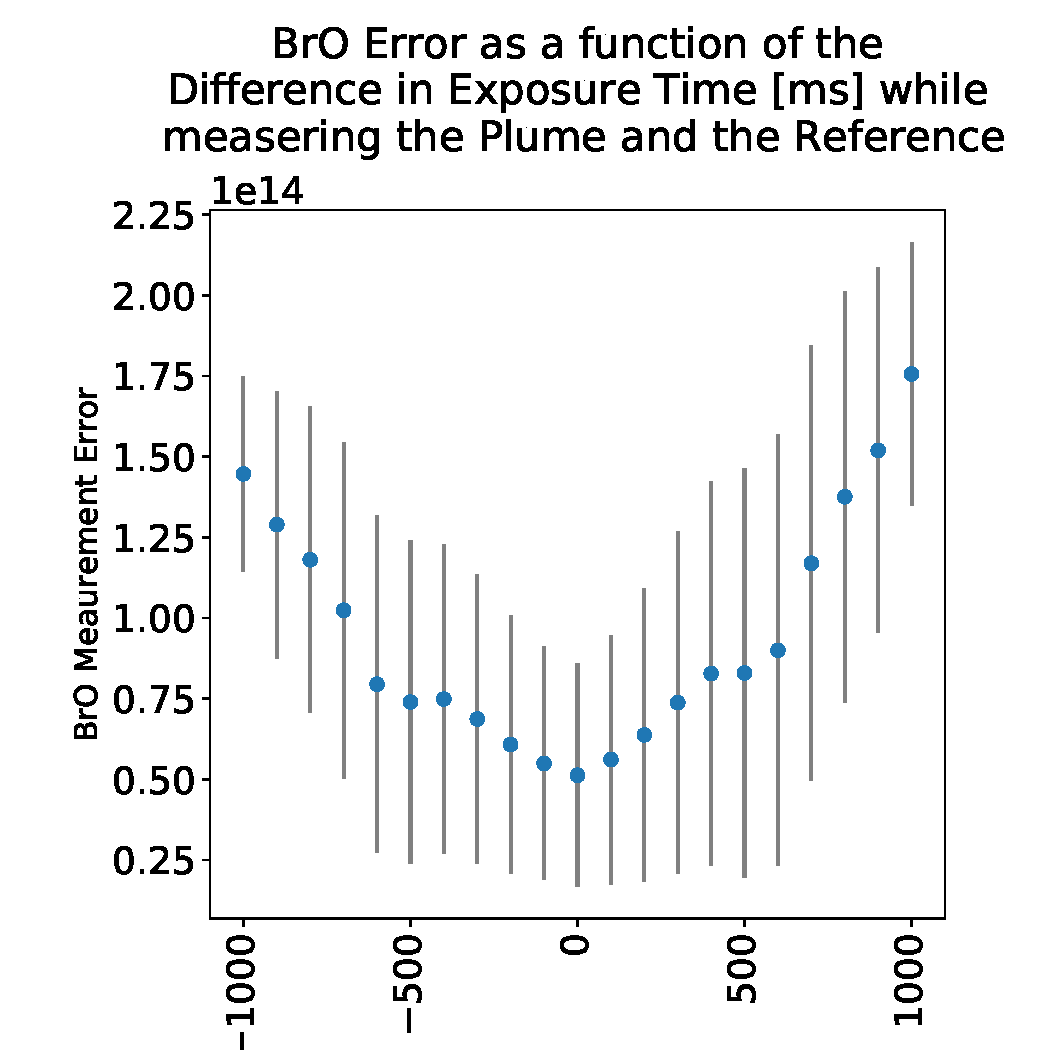
\includegraphics[width=0.49\textwidth]{Bilder/DiffExpTime_Nevad}}
	\caption{Titel unterm gesamten Bild}
	\label{fig:diffexptime}
\end{figure}
	\begin{itemize}
	\item The BrO Error increases with the exposure time differences as\\
	\begin{align*}
	\rightarrow&  BrO_{Error} = f(ext. P)+ 1.92\cdot10^{12}\cdot\frac{\Delta ET}{10^{-2}s} + \mathcal{O}\left(\right) & Tungurahua\\
	\rightarrow&  BrO_{Error} = f(ext. P)+ 1.0\cdot10^{13}\cdot\frac{\Delta T}{10^{-2}s} + \mathcal{O}\left(\right) & Nevado Del Ruiz\\
	\end{align*}
\end{itemize}
}

\frame{
	\frametitle{BrO Error Tungurhua /Nevado Del Ruiz}
	\begin{figure}[h]		
	\subfigure[Data of Tungurahua]{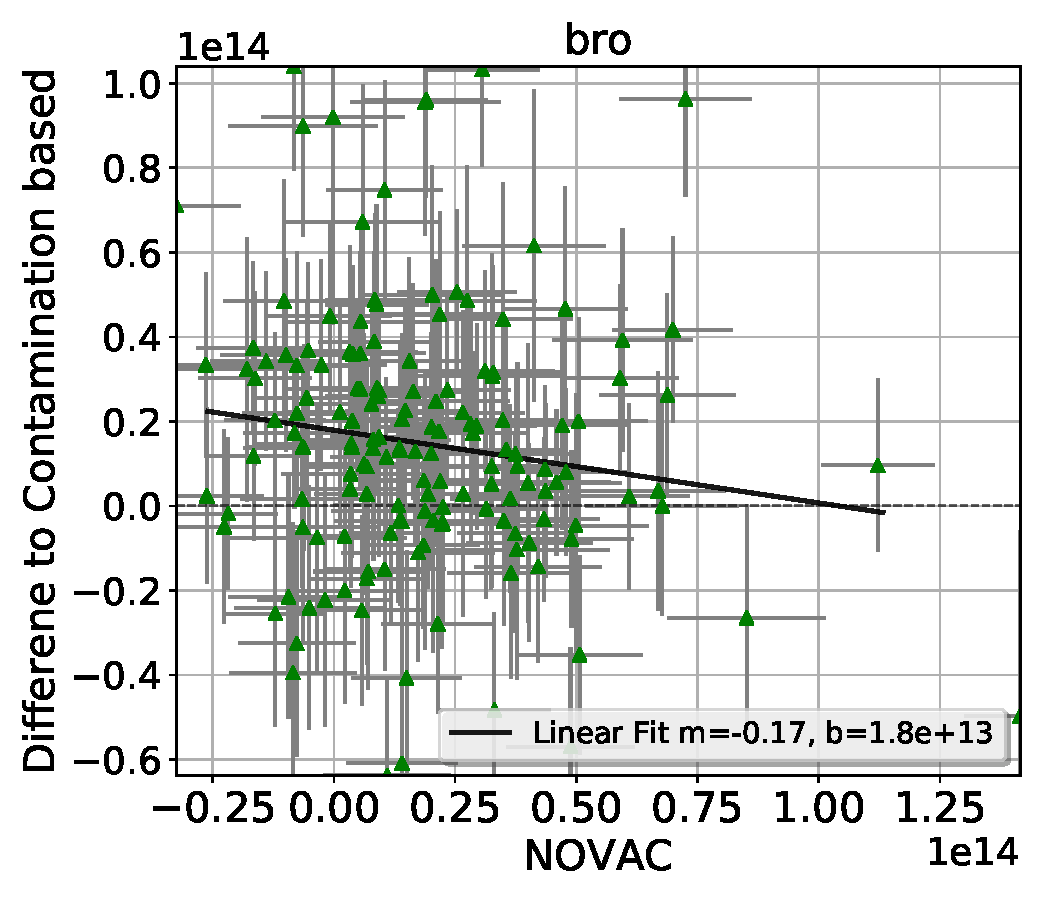
\includegraphics[width=0.49\textwidth]{Bilder/Tungurahua_Pic/tung_bro_diff_novac_conbased}}
	\subfigure[Data of Nevado Del Riz]{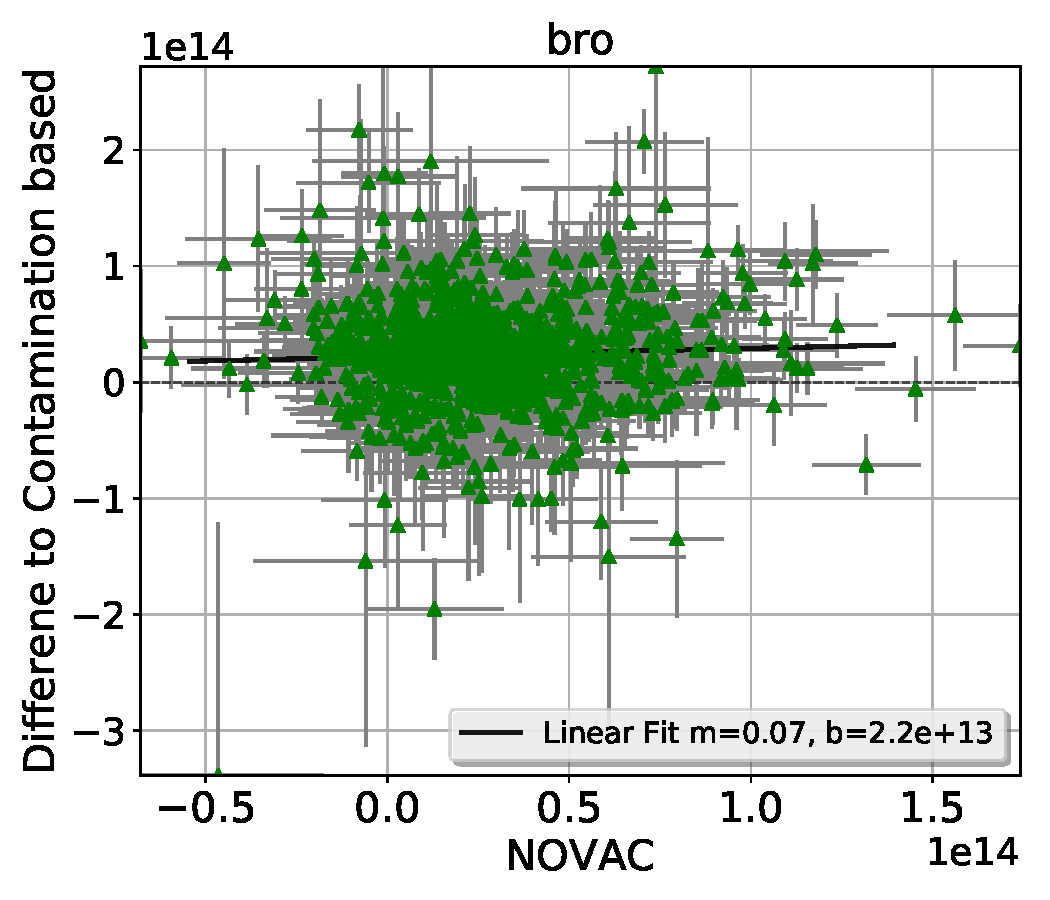
\includegraphics[width=0.49\textwidth]{Bilder/NevadoDelRuiz_Pic/bro_diff_novac_conbased}}
	\subfigure[Data of Tungurahua]{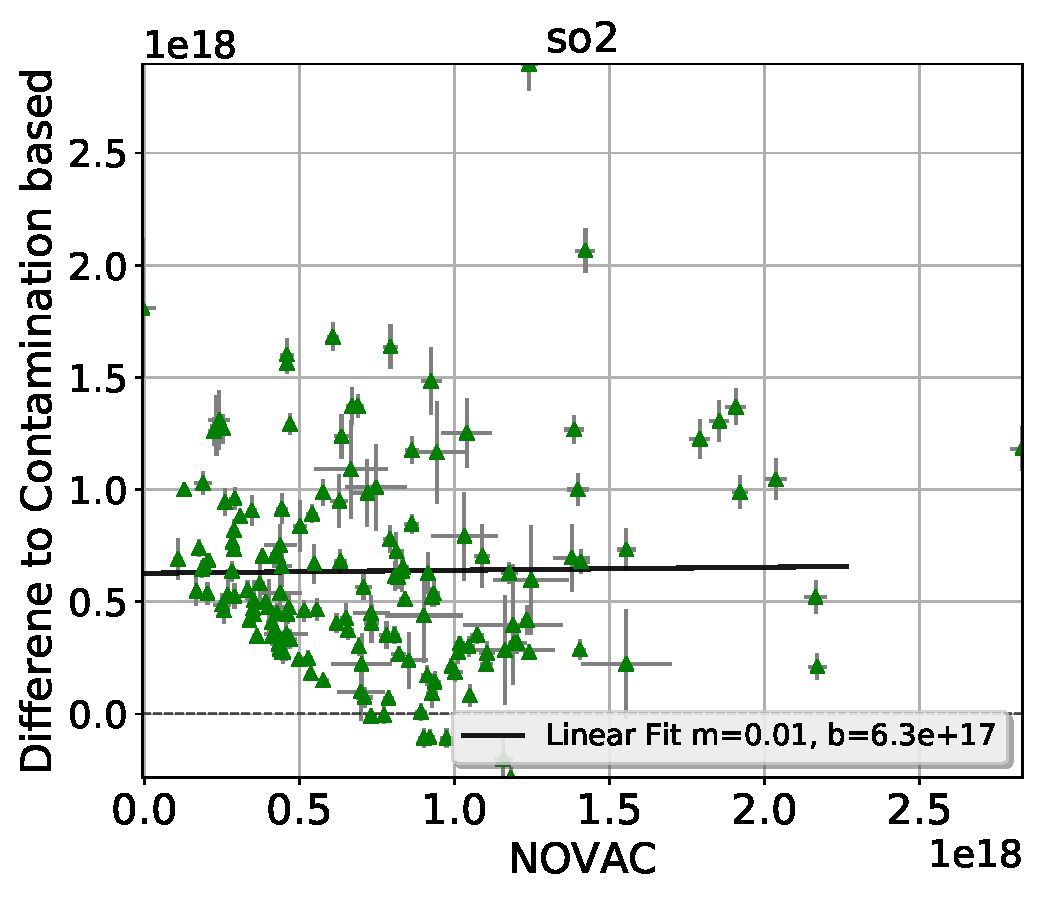
\includegraphics[width=0.49\textwidth]{Bilder/Tungurahua_Pic/tung_so2_diff_novac_conbased}}
	\subfigure[Data of Nevado Del Riz]{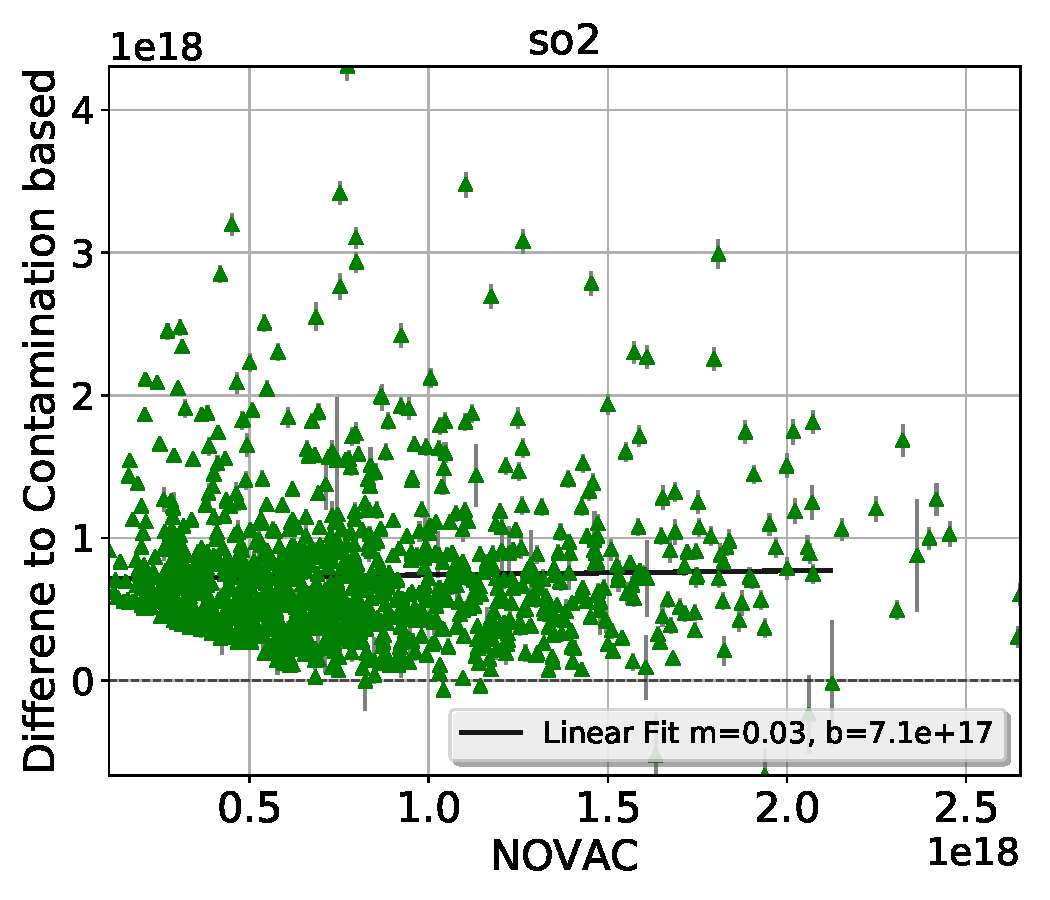
\includegraphics[width=0.49\textwidth]{Bilder/NevadoDelRuiz_Pic/so2_diff_novac_conbased}}
	\subfigure[Data of Tungurahua]{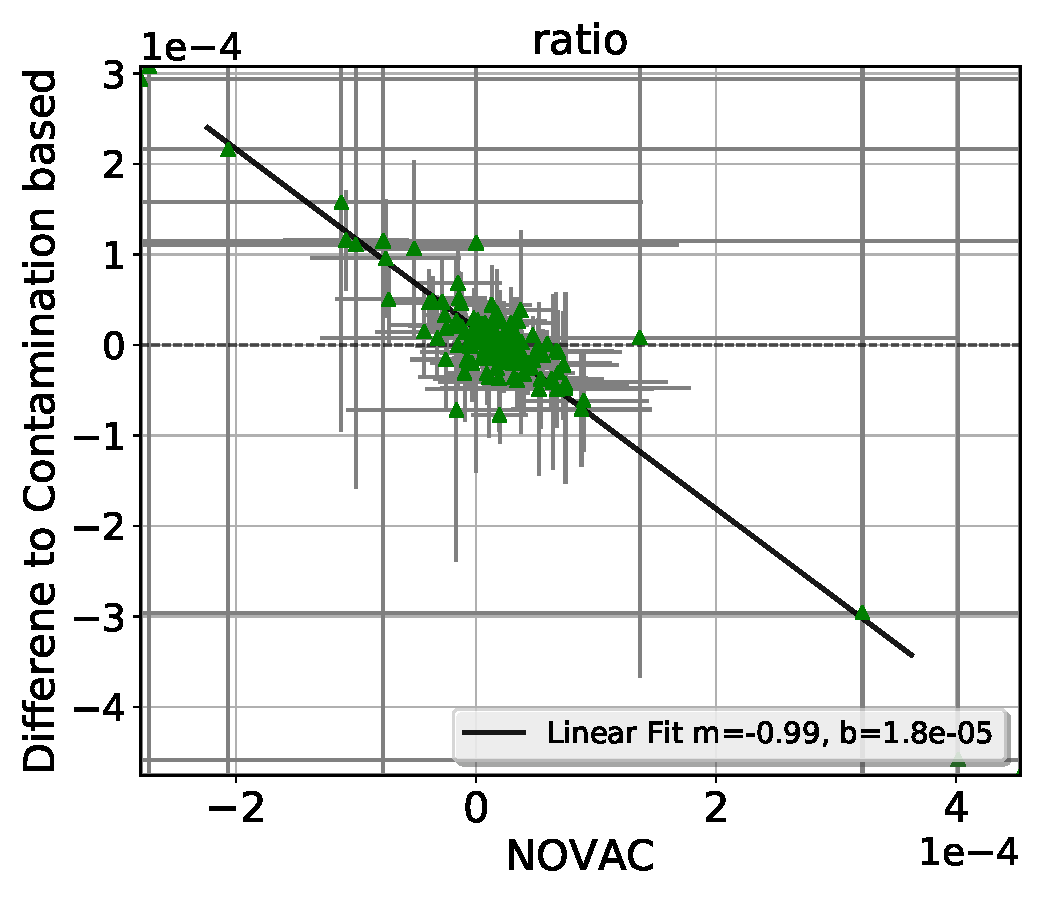
\includegraphics[width=0.49\textwidth]{Bilder/Tungurahua_Pic/tung_ratio_diff_novac_conbased}}
	\subfigure[Data of Nevado Del Riz]{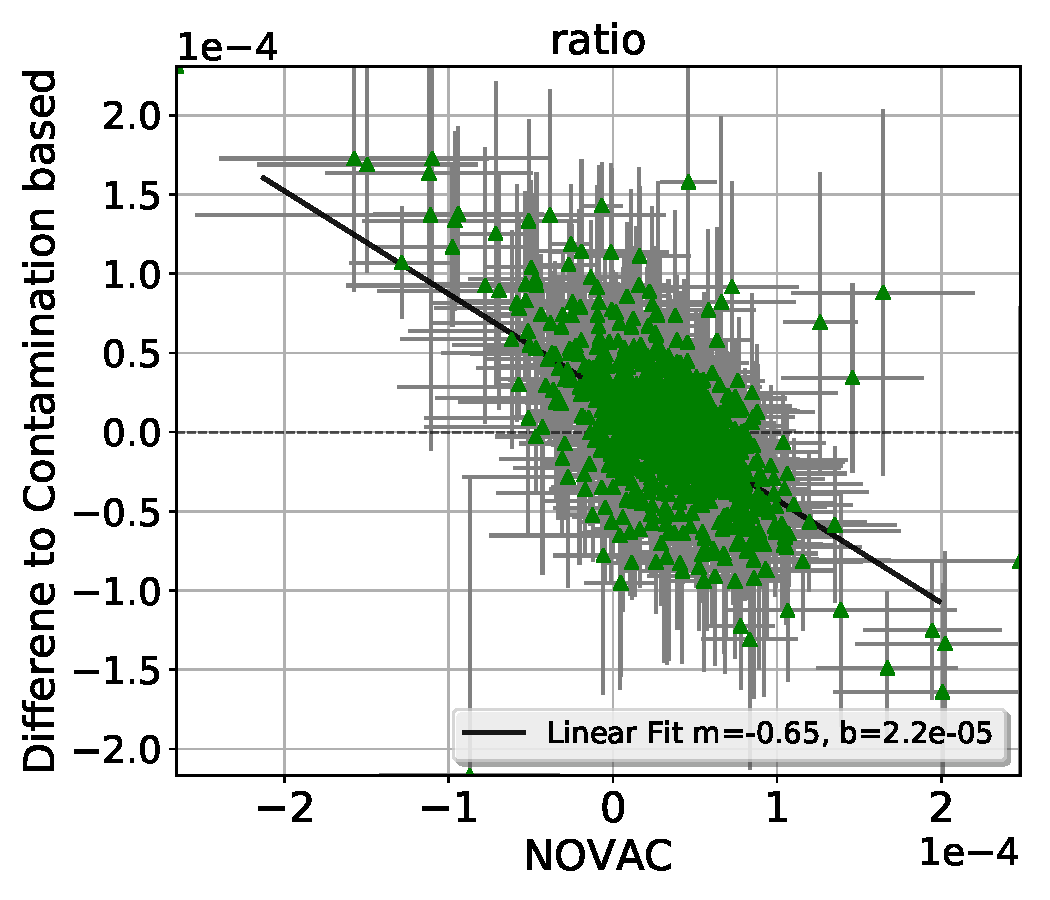
\includegraphics[width=0.49\textwidth]{Bilder/NevadoDelRuiz_Pic/ratio_diff_novac_conbased}}
	\caption{The dependency of the Difference between contamination based data and NOVAC to the data evaluated with the NOVAC data }
	\label{fig:diffcontbase}
\end{figure}
}
%------------------------------------------------
%	Calculations
%------------------------------------------------
\frame{
\frametitle{Calculations}
\begin{itemize}
\item linear approximation of the Data
\end{itemize}
\vspace{1cm}
	\begin{equation*}
	\Delta	\epsilon_{BrO} = a_{t}\cdot\Delta t+a_{temp}\cdot\Delta temp+a_{daytime}\cdot\Delta daytime +a_{coloridx}\cdot\Delta coloridx
	\end{equation*}
}
%------------------------------------------------
%	Actual fit in python
%------------------------------------------------
%\frame{
%\frametitle{Actual fit in python}
%\begin{itemize}
%\item 
%\end{itemize}
%}

%------------------------------------------------
%	Importance of Variables
%------------------------------------------------
\frame{
\frametitle{Calculations}
	Difference in Constants
	\begin{table}[h]
		\begin{tabular}{c|c|c}
			\toprule
			Constant& importance& deviation\\
			\toprule
			$a_{T}$& 0.661 & 29$\%$\\
			\midrule
			$a_{ET}$&0.011&164$\%$\\
			\midrule
			$a_{t}$& 0.133&50$\%$\\
			\midrule
			$a_{dt}$&0.138&	65$\%$\\
			\midrule
			$a_{c}$&0.061&136$\%$\\
			\bottomrule
		\end{tabular}
	\end{table}
}
%------------------------------------------------
%	Results
%------------------------------------------------
\frame{
\frametitle{Results}
}
%------------------------------------------------
%	SO2 Evaluation
%------------------------------------------------
\frame{
\frametitle{SO2 Evaluation}
\begin{multicols}{2}
\begin{itemize}
\item Increase if the SO2 column densities of: 84$\%$
\begin{itemize}
\item PILLATE: 62$\%$
\item HUAYRAPATE: 122$\%$
\item BAYUSHIG: 23$\%$ (\small{very view data})

\end{itemize}

%\item Faktor um den der Fehler w\"achst: 1.89
\item More Data relative to the NOVAC-Evaluation: 206$\%$ 
\end{itemize}

\begin{minipage}[t]{0.5\textwidth}
\footnote{Fit uses only data where SO2 column \\
density is higher than $7\cdot 10^{17}\frac{molec}{cm^2}$}
%\includegraphics[width=\textwidth]{./Bilder/SO2_comparison}
\end{minipage}
\end{multicols}
}
%------------------------------------------------
%	BrO Evaluation
%------------------------------------------------
\frame{
\frametitle{BrO Evalutaion}
\begin{multicols}{2}
\begin{itemize}
\item Instrument PILLATE
\begin{itemize}
\item Increase of BrO column density: 30$\%$
%\item Fehler:  1.67
%\item G\"ultige Daten: 80$\%$
\end{itemize}
\item Instrument HUAYRAPATE
\begin{itemize}
\item Increase of BrO column density: 87$\%$
%\item Fehler: 1.51
%\item G\"ultige Daten: 62$\%$
\end{itemize}
\item Instrument BAYUSHIG (\small{very view data})

\begin{itemize}
\item Increase of BrO column density: 35$\%$
%\item Fehler: 1.69
%\item keine g\"ultige Daten
\end{itemize}

\end{itemize}
\begin{minipage}[t]{0.5\textwidth}
\vspace*{-1cm}
%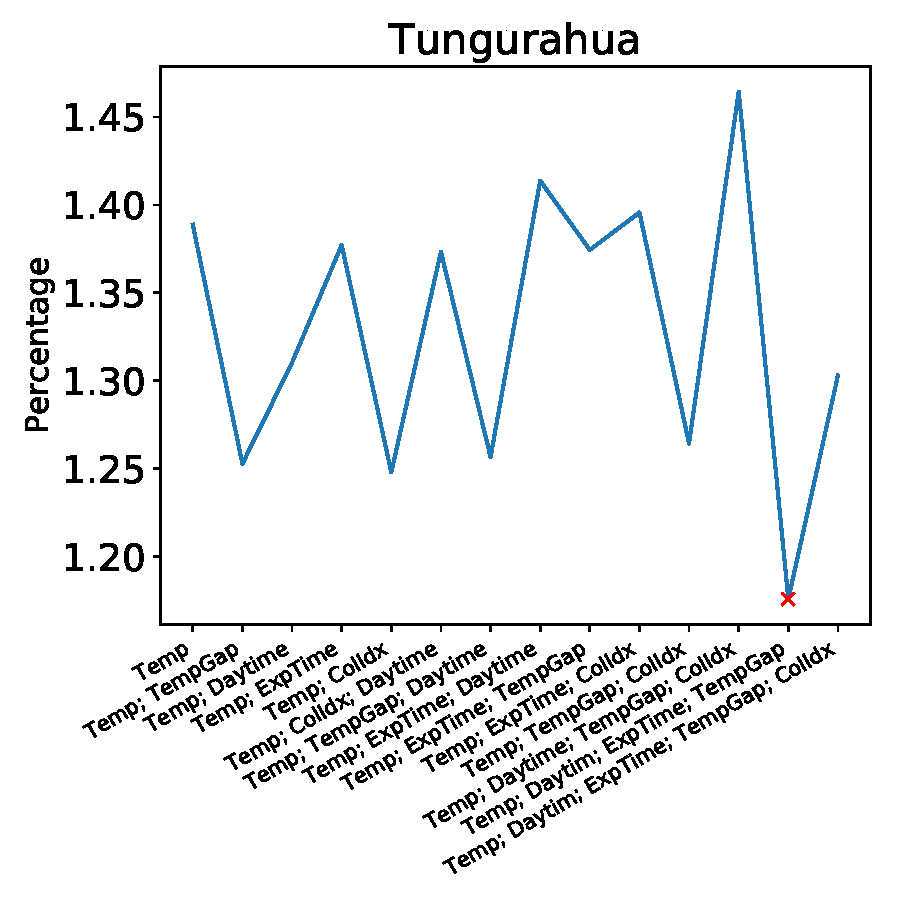
\includegraphics[width=0.9\textwidth]{./Bilder/Tungurahua}
\end{minipage}
\end{multicols}
}


\frame{
\frametitle{BrO Evaluation}
\begin{multicols}{2}
\begin{itemize}
\item Increase of BrO column density: 52$\%$
%\item More Data: 51$\%$
%\item More valid Data: 38$\%$ 
\item Factor the absolute error increases relative to the NOVAC-evaluation: 1.65
\item Factor the relative error increases relative to the optimal-results: 1.5
\end{itemize}

\begin{minipage}[t]{0.5\textwidth}
\footnote{Fit uses only data where SO2 column \\
density is higher than $7\cdot 10^{17}\frac{molec}{cm^2}$}
%\includegraphics[width=\textwidth]{./Bilder/BrO_comparison}
\end{minipage}
\end{multicols}
}
\frame{
\frametitle{Other Methods}
	\begin{table}[h]
%		\begin{tabular}{|p{2cm}|p{2.5cm}|p{1.5cm}|p{1.5cm}||p{1cm}|}
%		%	\toprule
%			&& Error & Amount of Data&davon gültig\\
%			\toprule
%			\multirow{2}{5em}{All Variables} 
%				& independent& 1.51 & 95$\%$&10,5$\%$\\
%				& dependent & 1.40&176 &14\\
%			\midrule
%			\multirow{2}{5em}{Exposure Time}
%					&  independent &1.47&174&18\\
%					& All &1.39&176&13\\
%			\midrule
%			\multirow{2}{5em}{Exp.Time u Coloridx}
%					&  independent &1.4&175&20\\
%					& All &1.35&176&13\\
%			\bottomrule
%		\end{tabular}
		\begin{tabular}{|p{2cm}|p{2.5cm}|p{1.5cm}|p{1.5cm}||p{1cm}|}
		%	\toprule
			&& Error & Amount of Data&valid data\\
			\toprule
			\multirow{2}{5em}{All Variables} 
				& independent& 1.51 & 95$\%$&10,5$\%$\\
				& dependent & 1.40&98$\%$ &8$\%$\\
			\midrule
			\multirow{2}{5em}{Exposure Time}
					&  independent &1.47&97$\%$&10$\%$\\
					& All &1.39&98$\%$&7$\%$\\
			\midrule
			\multirow{2}{5em}{Exp.Time u Coloridx}
					&  independent &1.40& 98$\%$&11\\
					& All & 1.35& 98$\%$&7$\%$\\
			\bottomrule
		\end{tabular}
	\end{table}
	$\bullet$ In the optimal results are 15$\%$ valid data
}

%------------------------------------------------
%	BrO Evaluation
%------------------------------------------------
\frame{
\frametitle{Ratio Evaluation}
\begin{multicols}{2}
\begin{itemize}
\item Decrease of gas ratio: 25$\%$
\begin{itemize}
\item PILLATE: 32$\%$
\item HUAYRAPATE: 12$\%$
\item BAYUSHIG: -6$\%$(\small{very view data})

\end{itemize}
%\item Difference zwischen den Berechnungsmethoden sink mit der Zunahme des Gas-Verh\"altnisses.
\end{itemize}

\begin{minipage}[t]{0.5\textwidth}
%\includegraphics[width=\textwidth]{./Bilder/Ratio_comparison}
\end{minipage}
\end{multicols}
}

\frame{
\frametitle{Total evaluation}
\begin{itemize}

\item More BrO Data: 51$\%$
\item More valid BrO Data: 38$\%$ 
%\item An average decrease of Ratio of 35$\%$

\end{itemize}
}
\frame{
	\frametitle{Tungurahua}
Menge an Daten insgesamt: --------------------------------------------------------- 5883 $\approx$ 1\\
Davon: Menge an daten (auch kontaminierten)(NOVAC Auswertung) über plume limit-- 712  $\approx$ 0.121\\
Davon: Menge an Daten, die nicht Kontaminiert sind:----------------------------- 5504 $\approx$ 0.936\\
Davon im Plume-limit:  ---------------------------------------------------- 599  $\approx$ 0.102\\
Davon über dem Detection Limit:-------------------------------------------- 36   $\approx$ 0.006\\
Davon sind kontaminiert: -------------------------------------------------------- 379  $\approx$ 0.064\\
Menge an kontamininierten Daten, mit NOVac ausgewertet, über plume limit:-- 114  $\approx$ 0.301\\
Menge an contaminierten Daten (Neue Auswertung) über plume limit----------- 185  $\approx$ 0.488\\
Dh in den kontaminierten daten sind mit NOVAC ausgewerteten daten 2.485 haeufiger ueber dem plume limit
}
\frame{
\frametitle{Nevado Del Ruiz}
Menge an Daten insgesamt:---------------------------------------------14005 $\approx$ 1\\
\hspace{0.5cm}Davon: Menge (auch cont)(NOVAC) \"uber plume limit----1818  $\approx$ 0.130\\
Davon: Menge an Daten, die nicht Kontaminiert sind:---------12613$\approx$ 0.901\\
Davon im Plume-limit:----------------------------------------------1238 $\approx$ 0.088\\
Davon über dem Detection Limit:-------------------------------234   $\approx$ 0.017\\
Davon sind kontaminiert:-------------------------------------------1392 $\approx$ 0.099\\
Menge an kontamininierten Daten, mit NOVAC, über plume limit:--------581  $\approx$ 0.417\\ 
Menge an contaminierten Daten (Neue Auswertung) über plume limit-----1140 $\approx$ 0.819\\

Dh in den kontaminierten daten sind mit NOVAC ausgewerteten daten 3.215 häufiger über dem plume limit}
\end{document}
